% Standalone PGFPlots fragment for \input into the paper body.
% Values are copied directly from the final ANN comparison for compile stability.
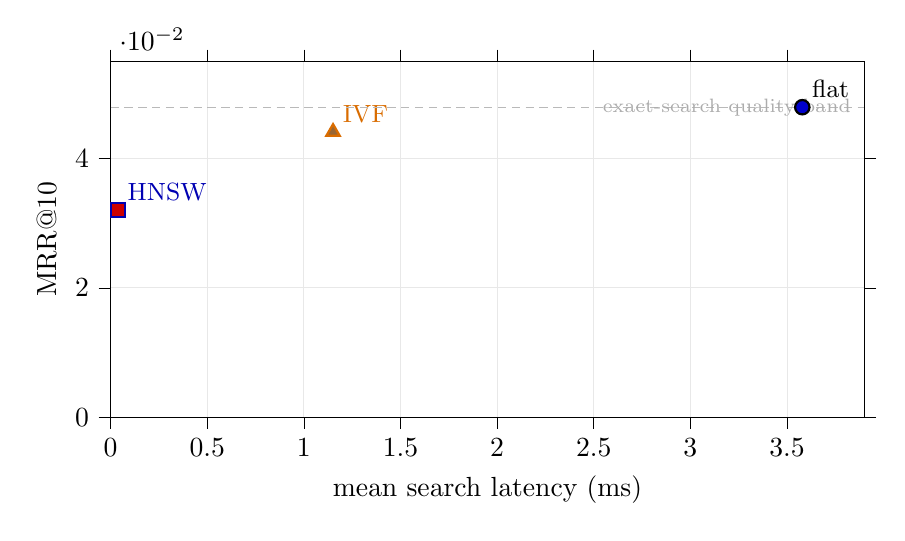
\begin{tikzpicture}
  \begin{axis}[
    width=0.92\linewidth,
    height=6.1cm,
    xlabel={mean search latency (ms)},
    ylabel={MRR@10},
    xmin=0,
    xmax=3.9,
    ymin=0.0,
    ymax=0.055,
    grid=both,
    major grid style={draw=gray!18},
    minor grid style={draw=gray!8},
    tick align=outside,
    tick style={black},
    legend style={draw=none, fill=none, at={(0.98,0.05)}, anchor=south east, font=\small},
    every axis plot/.style={line width=0.8pt},
    clip=false,
  ]
    % Exact search baseline.
    \addplot+[only marks, mark=*, mark size=2.6pt, color=black] coordinates {(3.5788,0.0479215)};
    \node[anchor=south west, font=\small] at (axis cs:3.5788,0.0479215) {flat};

    % HNSW and IVF.
    \addplot+[only marks, mark=square*, mark size=2.6pt, color=blue!70!black] coordinates {(0.0379,0.0320091)};
    \node[anchor=south west, font=\small, text=blue!70!black] at (axis cs:0.0379,0.0320091) {HNSW};

    \addplot+[only marks, mark=triangle*, mark size=2.8pt, color=orange!85!black] coordinates {(1.1511,0.0441068)};
    \node[anchor=south west, font=\small, text=orange!85!black] at (axis cs:1.1511,0.0441068) {IVF};

    % Readable contextual guides.
    \draw[densely dashed, gray!55] (axis cs:0,0.0479215) -- (axis cs:3.9,0.0479215);
    \node[anchor=east, font=\scriptsize, gray!65] at (axis cs:3.88,0.0479215) {exact-search quality band};
  \end{axis}
\end{tikzpicture}
